% Opener for December 9, 2026: three friends, three tiles (a who-has-which-tile puzzle on the Week 36 tiles)
% Build in a scratch directory: pdflatex three-tiles.tex, then copy to ../2026-12-09-opener.pdf
% Every puzzle here is checked for exactly one answer, with every clue needed, by three-tiles_check.py.
% Answer to all three-friend versions: Ana solid circle, Ben open triangle, Cy striped square (an allowed three).
\documentclass[11pt]{article}
\usepackage[letterpaper,margin=0.5in]{geometry}
\usepackage[T1]{fontenc}
\usepackage[default]{sourcesanspro}
\usepackage{tikz}
\usetikzlibrary{patterns}
\usepackage{ragged2e}
\pagestyle{empty}
\tikzset{fillo/.style={fill=white},fillh/.style={pattern=north east lines},fillf/.style={fill=black}}
\setlength{\parindent}{0pt}
% \tile{x}{y}{shape: c t s}{fill: o h f}{cell size}: a Week 36 tile in a grey frame
\newcommand{\tile}[5]{%
  \draw[gray!70,line width=.6pt] ({#1-#5/2},{#2-#5/2}) rectangle ({#1+#5/2},{#2+#5/2});
  \def\r{#5*0.3}%
  \ifx c#3\draw[line width=1pt,fill#4] (#1,#2) circle ({\r});\fi
  \ifx t#3\draw[line width=1pt,fill#4] (#1,{#2+\r*1.1}) -- ({#1+\r},{#2-\r*.85}) -- ({#1-\r},{#2-\r*.85}) -- cycle;\fi
  \ifx s#3\draw[line width=1pt,fill#4] ({#1-\r},{#2-\r}) rectangle ({#1+\r},{#2+\r});\fi}
% the nine tiles, rows by shape, columns by fill
\newcommand{\ninetiles}{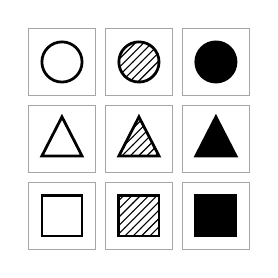
\begin{tikzpicture}[scale=0.85]
  \tile{0}{0}{c}{o}{1.0}\tile{1.15}{0}{c}{h}{1.0}\tile{2.3}{0}{c}{f}{1.0}
  \tile{0}{-1.15}{t}{o}{1.0}\tile{1.15}{-1.15}{t}{h}{1.0}\tile{2.3}{-1.15}{t}{f}{1.0}
  \tile{0}{-2.3}{s}{o}{1.0}\tile{1.15}{-2.3}{s}{h}{1.0}\tile{2.3}{-2.3}{s}{f}{1.0}
  \end{tikzpicture}}
% \friends{Ana,Ben,Cy}: an empty box under each name for the child to draw the tile
\newcommand{\friends}[1]{\begin{tikzpicture}
  \foreach \n [count=\i] in {#1}{\draw[line width=.8pt] ({\i*3.0},0) rectangle ({\i*3.0+2.2},2.2);
    \node[font=\large\bfseries] at ({\i*3.0+1.1},2.6) {\n};}
  \end{tikzpicture}}
\newenvironment{half}{\begin{minipage}[t][0.475\textheight][t]{\linewidth}\large\RaggedRight}{\end{minipage}}
\newcommand{\cutline}{\par\noindent\begin{tikzpicture}\draw[dashed,gray] (0,0)--(\linewidth,0);\end{tikzpicture}\par\vspace{0.3in}}
\newcommand{\heading}[1]{{\LARGE\bfseries #1}\hfill {\normalsize Name:} \rule{1.8in}{0.4pt}\par\medskip}
\newcommand{\twocol}[2]{\begin{minipage}[t]{0.58\linewidth}\vspace{0pt}#1\end{minipage}\hfill
  \begin{minipage}[t]{0.38\linewidth}\vspace{0pt}\centering #2\end{minipage}}
\newcommand{\mainpuzzle}{%
  \heading{Three friends, three tiles}
  Ana, Ben and Cy each picked one of these nine tiles. Their three shapes are all different,
  and their three fills are all different. Draw each friend's tile in their box.\par
  \medskip
  \twocol{%
  \begin{enumerate}\setlength{\itemsep}{4pt}
  \item Ana has a circle.
  \item Ben does not have a square.
  \item The solid tile is not a triangle.
  \item The striped tile is a square.
  \end{enumerate}}{\ninetiles}\par
  \smallskip
  \centerline{\friends{Ana,Ben,Cy}}\par
  \smallskip
  \textbf{Done?} Cross out clue 2. Find every answer now. Write a new clue that makes it exactly one again.}
\begin{document}
\begin{half}\mainpuzzle\end{half}
\cutline
\begin{half}\mainpuzzle\end{half}
\newpage
\begin{half}
\heading{Two friends, two tiles}
Ana and Ben each picked one of these tiles. One picked a circle and one picked a triangle.
One tile is open and one is solid. Draw each friend's tile in their box.\par
\medskip
\twocol{%
\begin{enumerate}\setlength{\itemsep}{6pt}
\item Ana has the circle.
\item The triangle is open.
\end{enumerate}\par
\medskip
\textbf{Done?} Try the three-friend puzzle.}{%
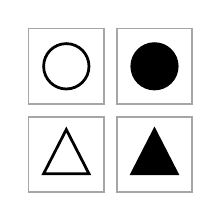
\begin{tikzpicture}[scale=0.8]\tile{0}{0}{c}{o}{1.2}\tile{1.4}{0}{c}{f}{1.2}\tile{0}{-1.4}{t}{o}{1.2}\tile{1.4}{-1.4}{t}{f}{1.2}\end{tikzpicture}}\par
\medskip
\centerline{\friends{Ana,Ben}}
\end{half}
\cutline
\begin{half}
\heading{Three friends, three tiles (harder)}
Ana, Ben and Cy each picked one of the nine tiles. Their three shapes are all different.
Their three fills are all the same, or all different. Draw each friend's tile in their box.\par
\medskip
\twocol{%
\begin{enumerate}\setlength{\itemsep}{4pt}
\item Ana has a circle.
\item Ben's tile is not striped.
\item The solid tile is not a triangle.
\item Someone has a striped square.
\end{enumerate}}{\ninetiles}\par
\smallskip
\centerline{\friends{Ana,Ben,Cy}}\par
\smallskip
\textbf{Done?} Change clue 2 to ``Ben does not have a square.'' Now there are two answers. Find them both.
\end{half}
\end{document}
